\cotefile{76}
\scanpage{51}
\deleted{Ainsi, si $S$ est l'un des sommets du cube $C(B,\sigma)$ -- correspondant aux sections de $B$ sur $I=B/\sigma$, alors \unsure{tout} $s\in S$ est l'intersection des facettes}

\uline{Corollaire} Soient $(B,\sigma)$, $(B',\sigma')$ deux \deleted{\unsure{basi}} maquettes de cubes, \deleted{Alors} définissant des cubes $C$, $C'$, de sorte que l'on a
\[
\operatorname{Isom}((B,\sigma),(B',\sigma'))\xrightarrow{\alpha}
\operatorname{Isom}_{\mathrm{aff}}(C,C')\xrightarrow{\beta}
\operatorname{Isom}_{\mathrm{ord}}(\operatorname{Comb}(C),\operatorname{Comb}(C'))
\]
Ces applications sont des isomorphismes. En particulier on a
\[
\begin{aligned}
\operatorname{Aut}((B,\sigma))&\xrightarrow{\sim}\operatorname{Aut}_{\mathrm{aff}}(C)\xrightarrow{\sim}\operatorname{Aut}_{\mathrm{ord}}(\operatorname{Comb}(C))\\
\shortparallel\qquad&\\[-2pt]
\text{commutant de }\sigma\qquad&\\
\text{dans }\unsure{\mathfrak S_B|\mathscr S_B}\qquad&\\
\mathrel{\rotatebox{90}{$\simeq$}}\ \text{non can.}\qquad&\\
\mathfrak S_I\cdot\{\pm1\}^{I}\qquad&
\end{aligned}
\]

\uline{Dém} On sait déjà que $\beta\alpha$ est un iso (histoire combinatoire -- cf cor. précédents). Il reste : prouver que $\beta$ l'est, On \unsure{en} sait déjà que $\beta$ est surjectif ($\beta\alpha$ bij), or il est injectif (car un isom $C\unsure{-|\to} C'$ est connu quand on connaît son effet sur les seuls pts extrémaux) -- g.g.

\uline{NB} Au lieu de $\operatorname{Isom}_{\mathrm{aff}}(C,C')$ on \deleted{peut} aussi d'écrire $\operatorname{Isom}_{\mathrm{proj}}(C,C')$

% slanted
\margin{\unsure{remonté|remonter}}
\uline{Corollaire} Les facettes du cube sont des cubes
% archive sheet number: 50
\scanpage{52}
\uline{\deleted{\unsure{Prop\textsuperscript{n}}}\unsure{Thme|Prop\textsuperscript{n}|Prop}} Le groupe $\operatorname{Aut}(C)$ est simplement transitif sur $\deleted{\unsure{\operatorname{Drap}}}\unsure{\operatorname{Rep}|\operatorname{Drap}}(C)$ (qui est \unsure{donc} un torseur \inserted{à g} sur $\operatorname{Aut}(C)$)

(On dit que $C$ est un pol (conv) \uline{régulier} quand il \deleted{\unsure{on}} \deleted{$\operatorname{Card}(\operatorname{Drap}(C))=2^n\cdot 2^{\unsure{n-1}}$} en est ainsi\ldots)

Le nb de facettes de dim $d+1$ contenant une facette donnée de dim $d$ est \deleted{$\unsure{2^d|2d}$} $(n-d)$, donc le nb des \deleted{drapeaux} \inserted{\unsure{rep.|drap.}} est
\[
2^n\cdot n\cdotn-1\cdot\ldots\,2\cdot1=2^n n!
\]
qui est aussi l'ordre de $\operatorname{Aut}(C)$. Il suffit de prouver que $\operatorname{Aut}(C)$ opère librement sur $\operatorname{Drap}(C)$, or c'est vrai pour tt polyèdre convexe :

\uline{Lemme} Soit $C$ un polyèdre convexe, $u$ un autom de $C$ fixant un drapeau de $C$. Alors $u$ est l'identité.

Récurrence sur $\dim C$. Pour $\dim C=0$, c'est triv. Soit $D=(F_0,\ldots,F_{n-1},F_n=C)$ le drapeau fixé. Par hyp. de récurrence, $u$ est l'identité sur $F_{n-1}$, car il fixe son \deleted{drapeau} \inserted{\unsure{rep.|drap.}} $(F_0,\ldots,F_{n-2},F_{n-1})$. Donc on a un autom \deleted{qui est} affine de $E_C=E$ qui \deleted{\unsure{f}}est l'identité sur un hyperplan $H=E_{F_{n-1}}$, et qui est d'ordre fini -- on voit facilement que c'est ou bien l'identité, ou bien une ``symétrie'' -- mais alors elle échange les deux $\frac12$ espaces déterminés par $H$, donc elle ne pourrait conserver $C$, OK.

\figure{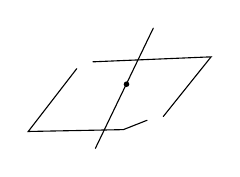
\begin{tikzpicture}[x=0.79cm,y=0.79cm,line cap=round]
\draw (0.78,1.01)--(0,0)--(1.53,0.03)--(1.91,0.18);
\draw (1.04,1.12)--(2.94,1.2)--(2.17,0.24);
\draw (1.08,-0.27)--(2.01,1.66);
\fill (1.58,0.76) circle (0.045);
\end{tikzpicture}}

\uline{Corollaire} Soit $C_0$ un cube de dim $n$, $D_0$ un drapeau du dit, \deleted{Al} $C$ un cube de dim $n$ Alors
\[
u\longmapsto u(D_0)\qquad\operatorname{Isom}(C_0,\deleted{\unsure{E}}C)\xrightarrow{\sim}\operatorname{Drap}(C)
\]
% archive sheet number: 51
\scanpage{53}
donc $\operatorname{Drap}(C)$ est un \uline{torseur à droite} sous $G_0=\operatorname{Aut}(\unsure{C^{0}|C_0})$ (et un torseur à gauche sous $G=\operatorname{Aut}(C)$, qui est le commutant de $G_0$\ldots)

Le foncteur
\diagram{\begin{tikzcd}[ampersand replacement=\&,row sep=1ex,column sep=large]
C\arrow[r] \& \operatorname{Drap}(C)\\
n\text{-Cubes}\arrow[r] \& G_0\text{-tors. à dr}
\end{tikzcd}}
est une équivalence de catégories

\uline{NB} $(C_0,\unsure{R_0|D_0})$ est défini à isom unique près -- donc aussi $G_0$. Si on veut, on prend pour $C_0$ le cube \unsure{standart|standard} $C_n$, \deleted{\unsure{avec le drapeau}} \inserted{qui du pt de} vue combinatoire correspond à $B=[1,n]\times\{\pm1\}$, avec comme drapeau celui défini par la section cte de valeur $1$, et ses restrictions aux sous-intervalles $[1,i]$ $(0\leq i\leq n)$. Ainsi on trouve un isom. can.
\[
\begin{aligned}
G_0&\simeq\{\pm1\}^n\cdot\unsure{\mathfrak S_n|\mathscr S_n}
\qquad\text{(produit }\tfrac12\text{ direct}\\
&\simeq\operatorname{Aut}(C_n)
\end{aligned}
\]
% archive sheet number: 52
\scanpage{54}
Symétrie du cube : c'est l'homothétie $\unsure{\varphi|q}\unsure{\mapsto|-}-\varphi$. Du pt de \unsure{vue|vu} combinatoire, c'est l'autom $I'\to\sigma I'$ dans l'ens des ``sections partielles'' de $B$ sur $I$. Du pt de \unsure{vue|vu} maquette du cube, c'est l'autom $\sigma$ de $(B,\sigma)$. C'est l'unique autom \inserted{$u$} ayant la

\deleted{\uline{Prop} Soient $F,F'$ deux facettes \inserted{fermées} non vides, Alors $F\cap F'\ne\varnothing$ \uline{ou} $F\cap\sigma F'\ne\varnothing$. (Ceci caractérise l'autom $\sigma$ ?) \deleted{Les facettes} Celà revient à ceci : Si $I',I''\subset B$ sont deux sections partielles de $B$ sur $I=B/\sigma$, alors ou bien}

propriété : si $F$ est une facette de codim un (une hyperfacette), alors $\sigma F$ est une hyperfacette ne \deleted{\unsure{se}} rencontrant pas $F$. Plus gén, pour \deleted{\unsure{deux}} \inserted{tte} facette \inserted{$F$} \deleted{de dim \unsure{$d$}} à part celle de dim $n$, $F$ et $\sigma F$ ne se rencontrent pas (en fait, les hyperplans d'appui ne se \deleted{\unsure{rencontrent}} pas et ils sont $\parallel$)

Aussi : le centre de $\operatorname{Aut}(C)$ est le groupe $\{1,\sigma\}$ [\uline{NB} si $n\geq3$, le centre de $\unsure{\mathfrak S_I|\mathscr S_I}$ est $\{1\}$ \ldots], donc $\sigma$ est l'unique élément central $\ne1$.

% slanted
\margin{\unsure{remonté|remonter}}
Nb de facettes de dim $d$ $(0\leq d\unsure{\leq|<}n)$
\[
c_d=\binom nd2^{n-d}
\]
On a la formule d'EP
\[
\begin{aligned}
\sum_0^n(-1)^d c_d&=\sum(-1)^d\binom nd2^{n-d}=(-1)^n\sum\deleted{\unsure{(-1)}}\binom nd1^d(-2)^{n-d}\\
&=(-1)^n(1-2)^n=1\qquad\text{i.e.}
\end{aligned}
\]
\[
\boxed{\sum_0^n(-1)^d c_d=1}
\]
(\uline{valable en fait pour tt polyèdre convexe de dim $n$!})
% archive sheet number: 53
\scanpage{55}
Ens. d'orientations du cube (ou de l'espace affine qu'il engendre, ce sera provisoirement notre définition ici\ldots)
\[
\omega_C\overset{\text{déf prov}}{\simeq}\omega_E\simeq
\unsure{\omega_I|\Omega_I}\wedge\bigwedge_{i\in I}B_i
\]
L'effet de $\sigma$ sur $\omega_C$ est $(-1)^n$, donc

\uline{Prop} L'antipodisme conserve l'orientation sss $n$ pair (donc \unsure{la|le} renverse \deleted{\unsure{si|ssi}} $n$ impair)

\uline{Cor} Soit $n$ impair, $\operatorname{Aut}(C)\simeq\operatorname{Aut}^+(C)\times\{\pm1\}$

\uline{NB} (Thème de méditation géométrique) : Soit $C$ un polyèdre convexe \deleted{dans un} \inserted{engendrant l'}espace affine $E$. Alors l'ens à 2 él. $\omega_E$ peut se décrire canoniquement en termes du polyèdre combinatoire $\operatorname{Comb}(C)$.

\uline{Indication} Une orientation \inserted{$\omega$} de $E$ permet de définir \inserted{l'ens $D(\omega)$} des ``\deleted{drapeaux} \inserted{repères} directs'' $F_0\subset F_1\subset\ldots\subset F_{n-1}\subset F_n=C$ (de facettes) du polyèdre $C$, et elle est définie par la connaissance de \deleted{\unsure{ces drapeaux}} \inserted{$D(\omega)$}. Il faut donc décrire, en termes de la seule structure d'ensemble ordonné de \inserted{$\Phi=$}$\operatorname{Comb}(C)$, quelles sont les parties de \deleted{$\operatorname{Comb}(C)$} \inserted{$D(\Phi)$} (ens des \deleted{drapeaux} \inserted{repères} de $\Phi$) qui sont de la forme $D(\omega)$ [définition combinatoire de l'orientation]. \uline{Solution} Soit $D^+\subset D$, $D^-=D\setminus D^+$, on veut que \inserted{les} $\sigma_i$ $(1\leq i\leq n)$ sur $D$ transforment $D^+$ en $D^-$ (donc $D^-$ en $D^+$\ldots). En fait, il y a \unsure{exactmt|exactt|exactement} 2 telles parties : $D^+$ et $D^-$ !
% archive sheet number: 54
\scanpage{56}
\margin{$\leftarrow$}Drapeaux d'un polyèdre convexe -- drapeaux d'un ens ordonné. Repères d'un polyèdre convexe

\uline{Prop.} Soit $C$ un polyèdre convexe, $\operatorname{Fac}(C)$ le polyèdre combinatoire, associé, $\operatorname{Rep}(C)=\operatorname{Rep}(\operatorname{Fac}(C))$ l'ens des repères. Alors les \deleted{applications} hom de gr
\[
\operatorname{Aut}_{\mathrm{aff}}(C)\xrightarrow{\alpha}\operatorname{Aut}_{\mathrm{ord}}(\operatorname{Fac}(C))\xrightarrow{\beta}\deleted{\unsure{S}}\operatorname{Aut}_{\mathrm{ens}}\operatorname{Rep}(C)
\]
\deleted{sont} injectives. Plus précisément pour $\beta$, $\operatorname{Aut}_{\mathrm{ord}}(\operatorname{Fac}(C))$ opère \uline{librement} sur $\operatorname{Rep}(C)$ (a fortiori, $\alpha$ l'étant aussi, $\operatorname{Aut}(C)$ opère librement)

En effet, $\alpha$ est inj. car un autom $u$ de $C$ est connu quand on connaît sa restriction aux pts extrémaux.

Soit $u$ un autom de $\Phi=\operatorname{Fac}(C)$, fixant un drapeau $(\unsure{x_0|F_0}\ldots x_{n-1},x_n)$. Par hyp de récurrence il \deleted{fixe $P_{x_{n-1}}$} est l'identité sur $\Phi_{x_{n-1}}$. D'autre part, s'il est l'identité sur un \deleted{facette} $P_{\deleted{\unsure{x_{n-1}}}x}$, $x$ une facette de dim $n-1$, et si $y$ est une facette telle que $x\wedge y$ est de dim $n-2$, alors il est l'identité sur $\Phi_y$ -- car il fixe un drapeau de $P_y$. Il faut voir que la rel. d'équiv. \inserted{sur $\unsure{\Phi_{n-1}}$} engendrée par ``$x$ et $y$ ont une facette de dim $n-2$ en commun'' est la relation grossière. \deleted{\unsure{Soit} en effet}

Argument topologique de connexité\ldots

\uline{Déf} $C$ \deleted{\unsure{est}} est dit polyèdre \uline{régulier} si $\operatorname{Aut}_{\mathrm{aff}}(C)$ est transitif (donc simplement transitif) sur $\operatorname{Rep}(C)$, homogène si pour tt $0\unsure{<|\leq}i\leq n\deleted{\unsure{+1|-1}}$, $\exists\,d_i\in\mathbb N$ tel que $\forall F\in\operatorname{Fac}_{i-1}(C)$, le cardinal de
% archive sheet number: 55
\scanpage{57}
l'ens des \deleted{facettes} $y\in\operatorname{Fac}_{i\deleted{\unsure{-1|n}}}(C)$ qui majorent $x$ soit $d_i$. Donc dans ce cas on a
\[
\operatorname{card}\operatorname{Rep}(C)=d_{\deleted{\unsure{1}}0}d_{\unsure{1}}\ldots d_{\unsure{n|n-1}}=d_0\ldots d_{n-1}
\]
(car $d_n=1$). \deleted{On a alors, si $N=\operatorname{Card}\operatorname{Aut}(C)$}\deleted{$N_c=\operatorname{Card}\operatorname{Aut}(\operatorname{Fac}(C))$}

\unsure{Evidemt|Evidemment} régulier $\Rightarrow$ homogène

\deleted{$N\mid N_c\mid\operatorname{card}D$ Evidemment, \unsure{si}}

Si
\[
\begin{aligned}
\deleted{\unsure{R}}N&=\operatorname{Card}\operatorname{Aut}(C)\\
N_c&=\operatorname{Card}\operatorname{Aut}(\operatorname{Fac}(C))\\
R&=\operatorname{Card}\operatorname{Rep}(C),
\end{aligned}
\]
on aura
\[
N\mid N_c\mid R
\]
et $C$ régulier $\Longleftrightarrow N=R$ (donc $N=N_c$), donc les autom combinatoires sont euclidiens) Donc dans ce cas on a une décomposition
\[
N=N_c=d_0\ldots d_n
\]

\noindent\rule{2em}{0.4pt}\par\nobreak\noindent\rule{2em}{0.4pt}

Orientation d'un polyèdre \inserted{\unsure{conv.|convexe}} $C$ : par définition on \unsure{en|sera} une orientation de l'espace affine $E_C$ qu'il engendre. \inserted{L'ens. de ses o. est de ordre 2} Mais on montre que l'ens $\omega(C)$ ne dépend, à isom canonique près, que de $\Phi(C)=\operatorname{Fac}(C)$ (polyèdre combinatoire, strict associé) Donc il y a \deleted{Isom}
\[
\begin{aligned}
\operatorname{Isom}_{\mathrm{ord}}(\Phi(C),\Phi(C'))&\longrightarrow\operatorname{Isom}(\omega(C),\omega(C'))\\
\operatorname{Aut}_{\mathrm{ord}}(\Phi(C))&\longrightarrow\{\pm1\}\qquad\text{(hom de groupes)}\\
&\hspace{2em}\shortparallel\\[-3pt]
&\hspace{1em}\unsure{\operatorname{Aut}_{\mathrm{Ens}}|\operatorname{Aut}_{\mathrm{ens}}}(\omega(C))
\end{aligned}
\]
Cas où $C$ admet un antipodisme : sa sign. est $(-1)^n$
% archive sheet number: 56
\scanpage{58}
Automorphismes du $n$-cube.

Considérons le $n$-cube de maquette $(B,\sigma)$, soit $I=B/\sigma$. Un automorphisme correspond à un autom. \inserted{$u$} de la maquette, induisant un autom $u_I$ de $I$, d'où une décomposition de $I$ en orbites
\[
 I=\coprod_{\deleted{\unsure{i}}\alpha\deleted{\unsure{\in A}}}I_\alpha
\]
($u_I$ est connu modulo conjugaison quand on connaît les cardinaux des $I_\alpha$, rangés par ordre croissant \ldots)

Soit $B_\alpha$ l'image inverse de $I_\alpha$, donc $B_\alpha$ est stable par $u$, \deleted{donc} \deleted{réunion d'orbites, \unsure{il y en a|dont|il y a des} chacune s'envoie \uline{sur} $I_\alpha$ avec un degré déterminé. Donc 2 cas à envisager $1^\circ$) $B_\alpha$ est une orbite. Soit $n_\alpha$} \inserted{la situation est $\sim$ somme des $(B_\alpha,u_\alpha=u|B_\alpha)$ sur $I_\alpha=B_\alpha/(\underbrace{\sigma|B_\alpha}_{\unsure{\sigma_\alpha}})$,} et on est amené à étudier chacun de ses \unsure{c.|cas} (Géométriquement, $C=\prod C_\alpha$, où $C_\alpha$ est le cube associé à $(B_\alpha,\unsure{\sigma_\alpha|\sigma}\deleted{\unsure{I_\alpha|\mid B_\alpha}}$, et $u=\prod u_\alpha$,\ldots). Celà nous ramène à étudier le cas où $u_I$ est transitif sur $I$.

$B$ est réunion d'orbites, dont chacune s'envoie sur $I$ (l'unique orbite \deleted{\unsure{$I_\alpha$}} de $u_I$ dans $I$), avec un degré déterminé. Donc il y a 2 cas

a) Deux orbites isomorphes à $I$ \deleted{\unsure{à lui|$\xrightarrow{\sim}$}} par $p:B\unsure{-|\to} I$. Alors, si \deleted{\unsure{$i$}} $\unsure{E|\varepsilon}$ est l'ens des 2 orbites, on a canoniquement
\[
 B\simeq E\times I,\qquad u=\mathrm{Id}_E\times\deleted{\unsure{\mathrm{Id}_I|\mathrm{Id}}}u_I
\]
% archive sheet number: 57
\scanpage{59}
où $u_{\unsure{E|\varepsilon}}$ est la \deleted{\unsure{autom}} perm. non identique de $E$ (\deleted{\unsure{toutes}} les fibres sont canoniquemt isom par les itérés de $u$)

b) Il y a une seule orbite dans $B$. Cette situation est aussi uniquement déterminée (modulo \inserted{$I$-}isom \deleted{\unsure{x}} une fois $I,u_I$ donnés, modulo isom une fois $n=\operatorname{card}I$ donné).

% slanted
\margin{``cas tordu''}
\diagram{\(\begin{array}{c@{\;}cccc}
 & &ub_1&&u^{\inserted{n-1}}\deleted{\unsure{u}}b_n\\[-2pt]
 & &\diagup\!\diagup&&\diagup\!\diagup\\[-2pt]
 &b_1&b_2&\ldots&b_n\\
 ub_n\,{=}&b'_1&b'_2&\ldots&b'_n\\
 \cline{2-5}
 &i_1&i_2&\ldots&i_n\\[-3pt]
 &&\shortparallel&&\shortparallel\\[-2pt]
 &&ui_1&&u^{\deleted{\unsure{n}}n-1}i_1
\end{array}\)}
\margin{\uline{NB} Classification des flèches $B\to\deleted{\unsure{B|\overline I}}I$ (\deleted{\unsure{surj.|$\operatorname{card}I$}}) d'\deleted{ens} $\mathbb Z$-ens. à \unsure{esp.|sp.} finis}

Ainsi, pour $n=\operatorname{Card}I$ fixé, les classes d'isom d'autom d'un $n$-cube (i.e. les classes de conjugaison d'éléments de $\operatorname{Aut}(C_n)=\{\pm1\}^n\cdot\unsure{\mathfrak S_n|\mathscr S_n}$) sont donnés par 2 suites d'entiers naturels
\[
\begin{aligned}
\alpha_1^+\ldots\alpha_n^+&\in\mathbb N\\
\alpha_1^-\ldots\alpha_n^-&\in\mathbb N
\end{aligned}
\]
\margin{$\alpha_i^+$ \inserted{($\alpha_i^-$) $=$} nb de cycles de long. $i$ de $u_I$ au dessus duquel il y a \unsure{un cycle} de long $i$ (resp. $2i$)}
satisfaisant
\[
\sum_1^{\unsure{n|\relbar}}i(\underbrace{\alpha_i^++\alpha_i^-}_{\alpha_i})=n
\]

\uline{Étude des facettes fixes} $(\ne\varnothing)$ \deleted{\illegible{1}} Correspondent aux parties non vides \inserted{$B'$} de $B$ qui a) stables par $I$ b) Sections partielles. Au dessus de chaque $I_\alpha$ correspondant au ``\unsure{bicycle|cycle|cas tordu}'',
% archive sheet number: 58
\scanpage{60}
$B'$ doit être vide, au dessus de chaque $I_\alpha$ non tordu, il est \deleted{\unsure{ou}} vide ou une des deux orbites de $B_\alpha$ sur $I_\alpha$ (trois cas), de sorte que le nb de \inserted{telles} facettes \deleted{\unsure{est}} (y inclus la facette $C$)
\[
\deleted{\prod_{\unsure{\alpha\ \text{non tordu}}}}3^{\sum\alpha_i^+}
\]

Les facettes de codim donnée $d$ correspondent aux parties $B'$ telles que \deleted{\unsure{l'image}} \inserted{$\operatorname{Card}B'=d$} \deleted{\unsure{est}}. On trouve, si $f_d$ est le nb de ces facettes
\[
\boxed{\sum_{i=0}^n f_d t^d=\prod_{i=1}^n(1+2t^i)^{\alpha_i^+}}
\]

\uline{Exemple} Automorphismes de $C_3$

\margin{$+,8$\\$-,8$}
a) Autom ``indécomposables''
\[
\left.
\begin{aligned}
1^\circ)\\2^\circ)
\end{aligned}
\right\}
\begin{aligned}
&\text{non tordu :}\quad e_1\unsure{-|\to}e_2-e_3\to e_1\quad\oplus\\
&\text{tordu}\qquad e_1-e_2-e_3\to -e_1\quad\ominus
\end{aligned}
\]
Le premier est une rotation \inserted{d'ordre 3} autour de la diagonale joignant $\deleted{\unsure{z}}e_1+e_2+e_3$ et $-e_1-e_2-e_3$. Il y a (sans compter la facette pleine) \uline{2 facettes} fixes, savoir les deux sommets précédents.

Le deuxième est d'ordre 6, \deleted{\unsure{Et}} c'est \inserted{(mod. conj.)} le produit du précédent avec l'antipodisme [\uline{NB} cette relation entre cas tordu et non tordu marche chaque fois que la dim $n$ est impaire]

b) Autom décomposables : deux cycles (dans $I$)

\deleted{$\unsure{\alpha_1^+,\alpha_1^+|\alpha_1^+\ \alpha_1^+}\ \unsure{f}\ \unsure{\alpha_2}$}
% archive sheet number: 59
\scanpage{61}
\margin{$-,6$}
$1^\circ$) Non \unsure{tordu|tordus} tous deux \quad $e_1\unsure{-|\to}e_1\quad e_2-e_3,\ e_3-e_2$

symétrie \unsure{autour|suivant} plan diagonal (\uline{ordre 2})

\margin{$+,6$}
$2^\circ$) 1 tordu, 2 non tordu \quad $e_1-{-e_1},\ e_2-e_3,\ e_3-e_2$

symétrie autour axe-arête \inserted{\unsure{conjugué|composée} au produit du préc. par antip.} (\uline{ordre 2})

\margin{$+,6$}
$3^\circ$) 1 non tordu, 2 tordu \quad $e_1-e_1,\ e_2\to e_3,\ e_3-{-e_2}$ (ordre 4)

rotation d'un quart de tour autour de l'axe perpendiculaire à \unsure{une|deux} face (axe-face)

\margin{$-,6$}
$4^\circ$) 1 tordu, 2 tordu \quad $e_1-{-e_1},\ e_2-e_3,\ e_3-{-e_2}$ (ordre 4)

(conjugué au précédent, suivi de \deleted{\unsure{symétrie}} \inserted{antipodisme})

c) Autom décomposables \unsure{à|.} trois cycles (déterminé par $\alpha_1^+$ et $\alpha_1^-$, $\alpha_1^++\alpha_1^-=3$)

\margin{$+,1$}
$1^\circ$) $\alpha_1^+=3$\qquad identité

\margin{$-,3$}
$2^\circ$) $\alpha_1^+=2$\qquad $e_1\to e_1,\ e_2-e_2,\ e_3\to -e_3$\qquad symétrie par rapport à plan \deleted{\unsure{d'axe}} coord.

\margin{$+,3$}
$3^\circ$) $\alpha_1^+=1$\qquad $e_1\to e_1,\ e_2-{-e_2},\ e_3-{-e_3}$\qquad sym. \unsure{par r.|par rapport} à axe coord

\margin{$-,1$}
$4^\circ$) $\alpha_1^+=0$\qquad antipodisme

En tout il y a $1\deleted{\unsure{4}}0$ classes \unsure{,|?}
\[
(10=2+4+4)
\]
\noindent\rule{\linewidth}{0.4pt}

\uline{Prop} Soit $u$ un autom de $C$ tel que pour tt sommet $x$, on ait $ux=\pm x$. Alors \inserted{(si $n\geq3$)} $u$ est l'identité ou l'antipodisme.

\unsure{Donc|D'où}
\[
\operatorname{Aut}(C)/(\pm1)\underset{\text{\uuline{inj}}}{\lhook\joinrel\longrightarrow}\operatorname{Aut}(\Phi_0(C)/\sigma)
\]
donc si $C$ de dim impaire
\[
\operatorname{Aut}^+(C)\unsure{\lhook\joinrel\relbar|\hookrightarrow}\operatorname{Aut}(\unsure{\Phi_0(C)|\Phi(C)})
\]
% archive sheet number: 60
\scanpage{62}
\uline{Corollaire} Soit $C$ un cube de dim 3. Alors
\[
\operatorname{Aut}^+(C)\xrightarrow{\sim}\operatorname{Aut}_{\mathrm{ens}}(\underbrace{\Phi_0(C)/\sigma}_{\text{ens. de card. 4}})
\]

\uline{Corollaire} Le foncteur $C\longmapsto\Phi_0(C)/\sigma$ est une équivalence de la catégorie des 3-cubes \inserted{\uline{orientés}} dans \deleted{\unsure{de dim 3|dans $\to$}} la cat. des ens. de card. 4 (en prenant comme morphismes les iso \ldots)

\uline{Cube (combinatoire) gauche}
\[
C=C(B,\sigma)\subset E=E_C=E(B,\sigma)
\]
cube. Considérons le quotient par la relation d'antipodisme, mais sur
\[
\partial\unsure{\hat C|\widetilde C|C^*|\overleftarrow C}=\coprod_{F\in\Phi^{**}(\deleted{\unsure{E}}C)}\overline F
\]
\[
\partial\hat C/\sigma\simeq E^*/\mathbb R^*=P(E)\qquad
\begin{aligned}&\text{espace projectif réel}\\&\text{de dim }n-1\end{aligned}
\]

La décomposition de $\partial\hat C$ en facettes donne une décomposition (où $C\overset{p}{\unsure{-|\to}}\partial C$ passage au quotient)
\[
\widetilde C\deleted{\unsure{-|=}}=\partial\hat C/\sigma
=\coprod_{F\in\Phi^{**}}p(F)=\coprod_{F\in\Phi^{**}}p(\overline F)
\]

NB Pour tte $F\in\Phi^{**}$, $\overline F\to P(E)$ est injectif

On a \deleted{$p(\overline F\cap\overline F')=p(\overline F)\cap p(\overline F')$ si $\overline F\cap\overline F'=$}
\[
p(\overline F)\cap p(\overline F')=
\begin{cases}
\varnothing\quad\text{si }\overline F\cap\overline F'=\varnothing\quad\text{et }\overline F\cap\sigma\overline F'=\varnothing\\
[p(\overline F)\cap p(\overline F')]\unsure{\cup|\mathbin{\dot\cup}}
[p(\overline F)\unsure{\cap\sigma|\cap|\overline{\cap}}p(\overline F')]\quad\text{sinon}\\
\deleted{\unsure{p(\overline F)\cap p(\sigma\overline F')\quad\text{si }\overline F\cap\sigma\overline F'\ne\varnothing}}
\end{cases}
\]
[\uline{NB} les relations $\overline F\cap\overline F'\ne\varnothing$ et $\overline F\cap\sigma\overline F'\ne\varnothing$ ne s'excluent pas]

\deleted{\unsure{i.e. si} $B\to I$ et $B',B''$ deux sections partielles}

et $p(\overline F)\cap p(\overline F')$ n'est pas néc. connexe : il est connexe sss \deleted{\unsure{une seule}} on n'a pas ces 2 relations à la fois)
% archive sheet number: 61
\scanpage{63}
\[
[p(\overline F)\subset p(\overline F')]\Longleftrightarrow\overline F\subset\overline F'
\]

\figure{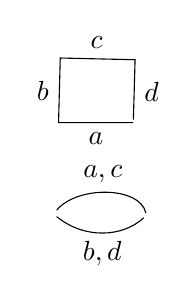
\begin{tikzpicture}[x=0.72cm,y=0.72cm,line cap=round]
\draw (1.32,.06)--(1.35,1.11)--(.03,1.14)--(0,0)--(1.31,0);
\node[below] at (.66,0) {$a$}; \node[left] at (0,.56) {$b$};
\node[above] at (.67,1.13) {$c$}; \node[right] at (1.34,.55) {$d$};
\draw (-.03,-1.54) .. controls (.33,-1.11) and (1.43,-1.12) .. (1.54,-1.59);
\draw (-.03,-1.66) .. controls (.45,-2.05) and (1.12,-2.03) .. (1.5,-1.68);
\node[above] at (.78,-1.23) {$a,c$}; \node[below] at (.77,-1.92) {$b,d$};
\end{tikzpicture}}

\uline{NB} On trouve une décomposition de $P(E)$ \deleted{\unsure{en}} en parties qui sont des cellules top -- les intersections entre deux telles cellules, si elles sont non vides, étant une cellule ou réunion de 2 cellules disjointes (donc ce n'est pas tjrs une cellule) Le schéma combinatoire de cette division cellulaire (ens ordonné des parties envisagées) est \deleted{\unsure{le}} $\Phi^{**}/\sigma\simeq$ ensemble ordonné opposé de $\unsure{\Psi^*|\Psi^\times|\Phi^*}/\sigma$, où $\Psi^*$ \unsure{est|$\to$} l'ens des sections partielles non vides de $B$ sur $I$.

Automorphismes des cubes gauches $(n\geq3)$
\[
\operatorname{Aut}(C)/\sigma\xrightarrow{\sim}\operatorname{Aut}_{\mathrm{proj}}\widetilde C\xrightarrow{\sim}\operatorname{Aut}_{\mathrm{ord}}(\Phi(\widetilde C))\qquad ?
\]

On sait déjà que la première \unsure{appliction|application} est injective, il est évident que la seconde l'est, le composé \deleted{\unsure{S|est}} est \deleted{\unsure{aussi}} surjectif ?

Si $n$ impair, on récupère $(\unsure{\mathcal X|\partial C|X|\mathcal H},\sigma)$ avec division cellulaire comme le rev. orienté canonique de $\widetilde C$, et tt autom de $\Phi(\widetilde C)$ est induit par un autom orienté de $\widetilde C$. Cas $n$ pair : à examiner \ldots
% archive sheet number: 62
